\chapter{Entropie et enthalpie libre de réaction}\label{ch:b2:reaction-free-energy}

Une poche de froid de sport contient un sachet d'eau et quelques cuillerées de nitrate
d'ammonium. On la presse, le sachet intérieur éclate, le sel se dissout et, en
quelques secondes, la poche est assez froide pour soulager une cheville foulée. La dissolution
absorbe de la chaleur --- elle est \omterm{def:b2:reaction-enthalpy:exothermic}{endothermique} --- et pourtant elle se produit d'elle-même,
jusqu'à son terme. L'enthalpie du chapitre précédent ne peut donc pas tout expliquer~:
une réaction ne va pas seulement «~vers le bas en chaleur~». La grandeur qui manque est
l'entropie, dont le second principe de la thermodynamique, rencontré en physique, fait le
juge de toute évolution spontanée. Ce chapitre tabule les entropies,
calcule l'entropie d'une réaction, et réunit enthalpie et entropie en
une seule fonction, l'\omterm{def:b2:reaction-free-energy:gibbs-energy}{enthalpie libre}, dont la dérivée par rapport à l'avancement décide du
sens de toute réaction à température et pression fixées.

\begin{recall}
En physique~: le second principe. Tout système possède une fonction d'état, son
entropie $S$ (extensive)~; lors d'une transformation d'un système fermé, $\dd S =
\delta Q/T_{\text{ext}} + \delta S_{\text{c}}$, où l'entropie créée
$\delta S_{\text{c}}$ est nulle pour une transformation réversible et positive
sinon~; pour un système fermé de composition fixée, $\dd U = T\dd S -
p\dd V$. \Cref{ch:b2:reaction-enthalpy}~: \omterm{def:b2:reaction-enthalpy:reaction-quantity}{grandeurs de réaction} $\Delta_r X =
(\partial X/\partial\xi)_{T,p}$ et \omterm{def:b2:reaction-enthalpy:standard-reaction-enthalpy}{enthalpies standard de réaction}. Le volume de
première année a énoncé, comme des lois «~qui découlent du second principe~», qu'une
réaction évolue jusqu'à ce que $Q = K^\circ$~; ce chapitre et les deux suivants les
démontrent.
\end{recall}

\begin{omfigure}
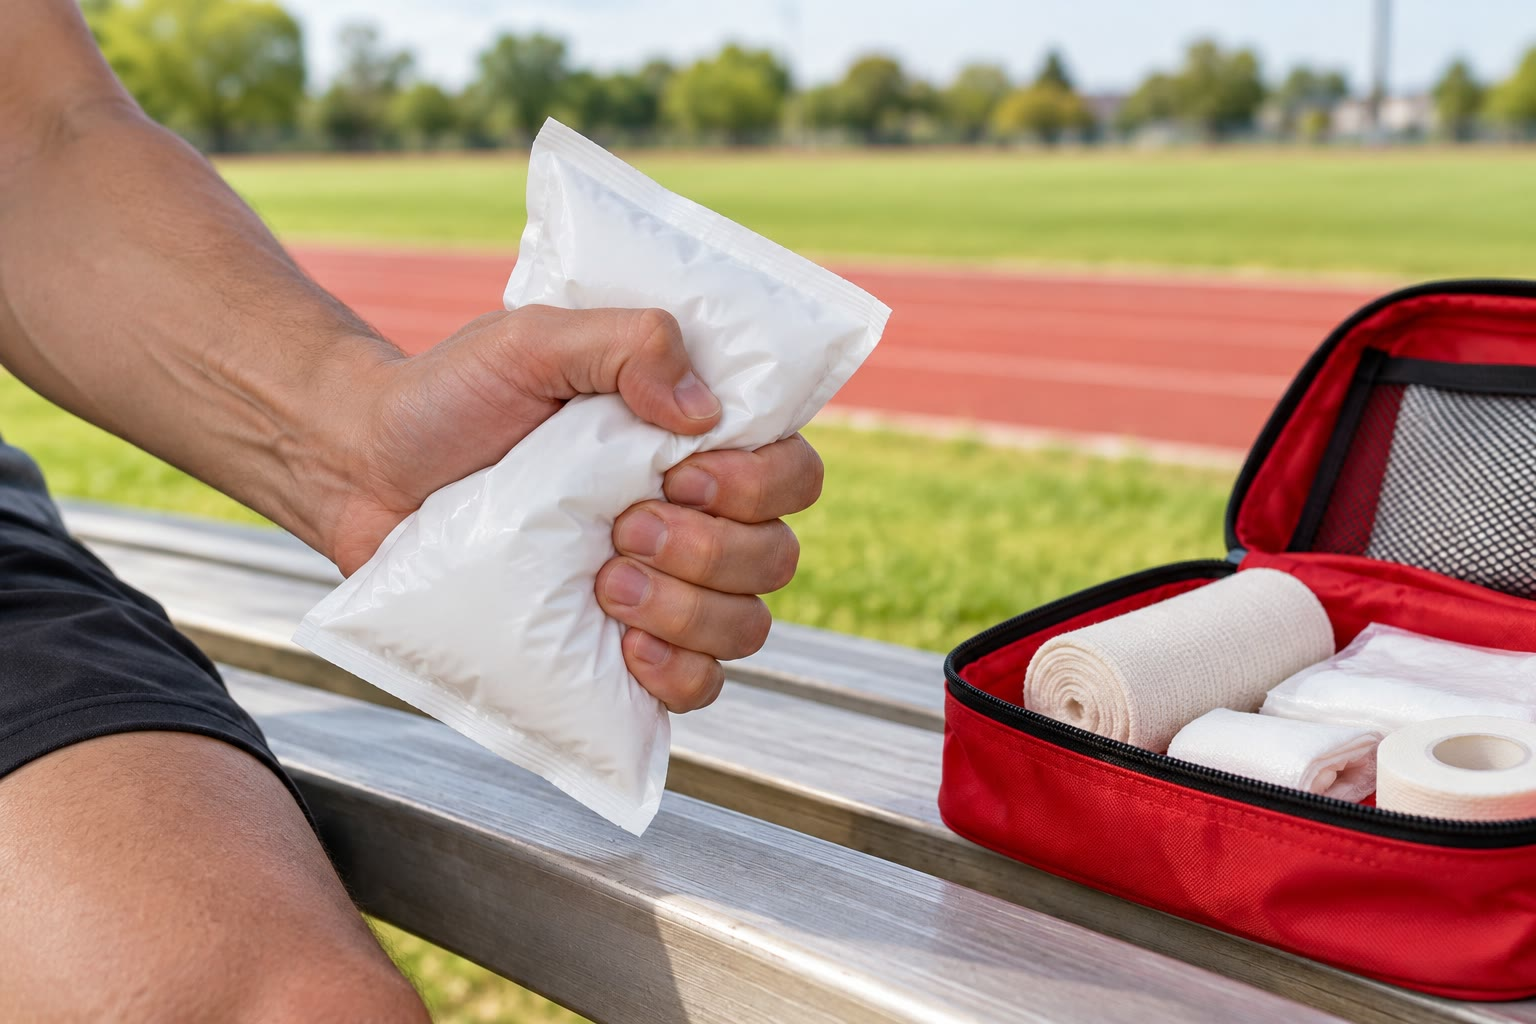
\includegraphics[width=0.55\linewidth]{images/book3/ai/b2-02-cold-pack.jpg}

{\small Une poche de froid~: lorsqu'on rompt son sachet intérieur, le nitrate d'ammonium
se dissout dans l'eau et la poche se refroidit. La dissolution est \omterm{def:b2:reaction-enthalpy:exothermic}{endothermique} et
spontanée~; son entropie explique pourquoi (\cref{ex:b2:reaction-free-energy:cold-pack}).}
\end{omfigure}

\section{Entropies standard et troisième principe}

Contrairement à l'enthalpie, l'entropie possède un zéro naturel.

\begin{theorem}[Troisième principe de la thermodynamique]\label{thm:b2:reaction-free-energy:third-law}
L'entropie d'un cristal pur et parfaitement ordonné tend vers zéro lorsque sa
température tend vers \qty{0}{K}.
\end{theorem}
\admitted

\begin{remark}[D'où vient le zéro]\label{rem:b2:reaction-free-energy:third-law}
Walther Nernst a énoncé en 1906 que les \omterm{def:b2:reaction-free-energy:reaction-entropy}{entropies de réaction} entre phases
condensées s'annulent lorsque $T \to 0$~; Max Planck en a tiré l'énoncé plus fort
ci-dessus. Son origine est statistique~: l'entropie dénombre les configurations
microscopiques compatibles avec l'état d'un système, et un cristal parfait
à \qty{0}{K} n'en possède qu'une. Ce dénombrement est fait dans le volume de troisième année,
à l'aide des fonctions de partition.
\end{remark}

\begin{definition}[Entropie molaire standard]\label{def:b2:reaction-free-energy:standard-entropy}
L'\emph{entropie molaire standard}\index{entropie molaire standard}
$S^\circ_m(T)$ d'une substance est l'entropie d'une mole de celle-ci dans son
état standard à la température $T$, le zéro étant celui du troisième principe.
Contrairement à $\Delta_f H^\circ$, c'est une grandeur absolue, positive pour toute
substance, éléments compris.
\end{definition}

\begin{proposition}[Entropie absolue à partir des capacités thermiques]\label{prop:b2:reaction-free-energy:absolute-entropy}
En chauffant une substance sous la pression constante $p^\circ$ de \qty{0}{K} à $T$,
\[
  S^\circ_m(T) = \int_0^T\frac{C^\circ_{p,m}(T')}{T'}\,\dd T' +
  \sum_{\text{transitions}}\frac{\Delta_{\text{trs}}H^\circ}{T_{\text{trs}}} ,
\]
l'intégrale étant prise dans chaque phase sur son domaine de température.
\end{proposition}

\begin{proof}
Chauffer la substance de façon réversible à pression constante~: $\delta S_{\text{c}} =
0$ et $\delta Q = \dd H = C_p\,\dd T$, donc $\dd S = C_p\,\dd T/T$. Lors d'un
changement d'état (fusion, ébullition), la température reste égale à $T_{\text{trs}}$
pendant que la chaleur $\Delta_{\text{trs}}H$ est reçue de façon réversible~: l'entropie
fait un saut de $\Delta_{\text{trs}}H/T_{\text{trs}}$. Il reste à additionner les morceaux à partir du
zéro du troisième principe.
\end{proof}

\begin{omfigure}
\begin{tikzpicture}
\begin{axis}[
  width=0.8\linewidth, height=6.2cm, xmin=0, xmax=1500, ymin=0, ymax=210,
  axis x line=bottom, axis y line=left, xlabel={$T$ (K)},
  ylabel={$S^\circ_m$ du zinc (\unit{J/(K.mol)})},
  xtick={0,250,500,750,1000,1250,1500},
  tick label style={font=\small}, label style={font=\small}, clip=false]
\addplot[omDef, very thick, smooth] table[x=T, y=S] {figdata/out/bachelor-2-standard-entropy-solid.dat};
\addplot[omProp, very thick] table[x=T, y=S] {figdata/out/bachelor-2-standard-entropy-liquid.dat};
\addplot[omThm, very thick] table[x=T, y=S] {figdata/out/bachelor-2-standard-entropy-gas.dat};
\draw[densely dashed, gray] (axis cs:692.73,64.6) -- (axis cs:692.73,75.2);
\draw[densely dashed, gray] (axis cs:1180.2,91.9) -- (axis cs:1180.2,189.6);
\node[omDef, font=\small, anchor=south east] at (axis cs:600,60) {solide};
\node[omProp, font=\small, anchor=north west] at (axis cs:850,78) {liquide};
\node[omThm, font=\small, anchor=south] at (axis cs:1350,192) {gaz};
\node[font=\scriptsize, anchor=west, align=left] at (axis cs:700,110) {fusion, $+10.6$\\ à \qty{692.7}{K}};
\node[font=\scriptsize, anchor=east, align=right] at (axis cs:1170,150) {ébullition,\\ $+97.7$ à\\ \qty{1180.2}{K}};
\end{axis}
\end{tikzpicture}

{\small \omterm{def:b2:reaction-free-energy:standard-entropy}{Entropie molaire standard} du zinc à partir du zéro du troisième principe. Elle croît
avec la température à mesure que le métal emmagasine de la chaleur, puis fait un saut au point de
fusion de $\Delta_{\text{fus}}H/T_{\text{fus}}$ et, bien plus grand, au point
d'ébullition de $\Delta_{\text{vap}}H/T_b$~: un gaz est bien plus désordonné qu'un
liquide.}
% ledger: s0T:Zn_crl.0, s0T:Zn_crl.298.15, s0T:Zn_cr.692, s0T:Zn_l.692, s0T:Zn_l.1180, s0T:Zn_g.1180, hT:Zn_cr.692, hT:Zn_l.692, hT:Zn_l.1180, hT:Zn_g.1180, dfh:Zn_g (curve in figdata/bachelor-2/standard-entropy.py)
\end{omfigure}

La figure donne des ordres de grandeur à retenir. À température ambiante,
un métal ou un cristal dur possède quelques dizaines de
\unit{J/(K.mol)}, un liquide une centaine, un gaz cent à trois cents~;
la fusion ajoute un peu, l'ébullition beaucoup. Les \omterm{def:b2:reaction-free-energy:standard-entropy}{entropies molaires standard}
utilisées dans ce volume sont tabulées avec les enthalpies de formation.

\section{Entropie de réaction}

\begin{definition}[Entropie de réaction]\label{def:b2:reaction-free-energy:reaction-entropy}
L'\emph{entropie de réaction}\index{entropie de reaction@entropie de réaction} est $\Delta_r S =
(\partial S/\partial\xi)_{T,p}$, et l'\emph{entropie standard de
réaction}\index{entropie standard de reaction@entropie standard de réaction} est $\Delta_r S^\circ(T) =
\sum_i\nu_iS^\circ_{m,i}(T)$, en \unit{J/(K.mol)}.
\end{definition}

Comme les entropies standard sont absolues, aucune réaction de formation n'est nécessaire~:
les éléments comptent avec leur propre entropie.

\begin{example}[Trois entropies de réaction]\label{ex:b2:reaction-free-energy:entropies}
À \qty{298.15}{K}~:
\begin{itemize}
  \item \ce{CaCO3(s) -> CaO(s) + CO2(g)}~: $\Delta_r S^\circ = 39.75 + 213.79 -
        92.9 = \qty{+160.6}{J/(K.mol)}$, un gaz formé à partir d'un solide~;
  \item \ce{N2(g) + 3H2(g) -> 2NH3(g)}~: $\Delta_r S^\circ = 2(192.77) -
        191.61 - 3(130.68) = \qty{-198.1}{J/(K.mol)}$, quatre molécules de gaz
        qui deviennent deux~;
  \item \ce{N2O4(g) -> 2NO2(g)}~: $\Delta_r S^\circ = 2(240.03) - 304.38 =
        \qty{+175.7}{J/(K.mol)}$.
\end{itemize}
% ledger: s0:CaCO3_cr, s0:CaO_cr, s0:CO2_g, s0:N2_g, s0:H2_g, s0:NH3_g, s0:N2O4_g, s0:NO2_g (computed in figdata/bachelor-2/thermo-data.py)
\end{example}

\begin{proposition}[Le signe d'une entropie de réaction]\label{prop:b2:reaction-free-energy:sign-rule}
Lorsque des gaz interviennent, le signe de $\Delta_r S^\circ$ est en général celui de
$\Delta\nu_{\text{gaz}} = \sum_{\text{gaz}}\nu_i$, et sa valeur est d'environ
\qty{100}{} à \qty{200}{J/(K.mol)} par mole de gaz formée ou consommée. Lorsque
$\Delta\nu_{\text{gaz}} = 0$, ou qu'aucun gaz n'intervient, $\Delta_r S^\circ$ est
petite et son signe doit être calculé.
\end{proposition}

\begin{proof}[Justification]
L'entropie molaire d'un gaz à \qty{298}{K} est comprise entre 130 et
\qty{300}{J/(K.mol)}, celle d'un solide ou d'un liquide vaut quelques dizaines~: former ou
consommer une mole de gaz l'emporte sur toute autre contribution. C'est une
règle pratique, non un théorème~: la dissolution d'un sel, sans aucun gaz, peut
encore changer l'entropie d'une centaine de \unit{J/(K.mol)}.
\end{proof}

\begin{method}[Prévoir le signe de $\Delta_r S^\circ$]\label{met:b2:reaction-free-energy:entropy-sign}
\begin{enumerate}
  \item Compter $\Delta\nu_{\text{gaz}}$~: s'il n'est pas nul, il donne le
        signe.
  \item Sinon, comparer l'ordre des états~: dissoudre un cristal,
        fondre, couper une molécule en deux morceaux augmentent l'entropie~;
        précipiter, solidifier, réunir deux molécules en une seule la diminuent.
  \item Lorsque la décision importe, calculer $\sum_i\nu_iS^\circ_{m,i}$.
\end{enumerate}
\end{method}

Le volume de première année en a rencontré une conséquence~: une élimination produit plus de molécules
qu'une substitution avec les mêmes réactifs (l'alcène, le groupe partant
et la base protonée, contre le produit de substitution et le groupe
partant). Son \omterm{def:b2:reaction-free-energy:reaction-entropy}{entropie de réaction} est plus grande, et le terme entropique, qui croît
avec la température comme le montre la section suivante, explique pourquoi la chaleur favorise
l'élimination au détriment de la substitution.

\section{L'enthalpie libre}

\begin{definition}[Enthalpie libre]\label{def:b2:reaction-free-energy:gibbs-energy}
L'\emph{enthalpie libre}\index{enthalpie libre} (ou énergie de Gibbs) d'un système
est la fonction d'état $G = H - TS$, extensive, en joules.
\end{definition}

\begin{definition}[Enthalpie libre de réaction]\label{def:b2:reaction-free-energy:reaction-gibbs}
L'\emph{enthalpie libre de réaction}\index{enthalpie libre de reaction@enthalpie libre de réaction} est $\Delta_r G
= (\partial G/\partial\xi)_{T,p}$, et l'\emph{enthalpie libre standard de
réaction}\index{enthalpie libre standard de reaction@enthalpie libre standard de réaction} est $\Delta_r G^\circ(T) =
\sum_i\nu_iG^\circ_{m,i}(T)$, toutes deux en \unit{kJ/mol}.
\end{definition}

\begin{proposition}[Terme enthalpique et terme entropique]\label{prop:b2:reaction-free-energy:g-h-s}
$\Delta_r G = \Delta_r H - T\Delta_r S$, et $\Delta_r G^\circ = \Delta_r
H^\circ - T\Delta_r S^\circ$.
\end{proposition}

\begin{proof}
Dériver $G = H - TS$ par rapport à $\xi$ à $T$ et $p$ fixées~: $T$
est une constante pour cette dérivation.
\end{proof}

\begin{proposition}[Différentielle de $G$ pour un système en réaction]\label{prop:b2:reaction-free-energy:dG}
Pour un système fermé siège d'une seule réaction, à $T$ et
$p$ uniformes,
\[
  \dd G = V\,\dd p - S\,\dd T + \Delta_r G\,\dd\xi .
\]
\end{proposition}

\begin{proof}
$G(T, p, \xi)$ a pour différentielle totale $\dd G = (\partial G/\partial
T)_{p,\xi}\dd T + (\partial G/\partial p)_{T,\xi}\dd p + \Delta_r G\,\dd\xi$.
Les deux premières dérivées partielles sont prises à composition fixée~: ce sont
celles d'un système fermé de composition fixée, pour lequel la physique donne
$\dd U = T\dd S - p\dd V$, de sorte que $\dd G = \dd U + p\dd V + V\dd p - T\dd S
- S\dd T = V\dd p - S\dd T$. D'où $(\partial G/\partial T)_{p,\xi} = -S$
et $(\partial G/\partial p)_{T,\xi} = V$.
\end{proof}

\section{Le critère d'évolution}

\begin{theorem}[Critère d'évolution]\label{thm:b2:reaction-free-energy:evolution}
Dans un système fermé maintenu à température et pression constantes, qui n'échange aucun
autre travail que celui des forces de pression, une réaction ne peut avancer que dans
le sens qui rend
\[
  \Delta_r G\,\dd\xi \leq 0 ,
\]
l'égalité étant réalisée à l'équilibre. Si $\Delta_r G < 0$, la réaction évolue dans le
sens direct~; si $\Delta_r G > 0$, elle évolue dans le sens inverse~; et le système est à
l'équilibre lorsque $\Delta_r G = 0$.
\end{theorem}

\begin{proof}
Considérons une transformation infinitésimale à $T$ et $p$ uniformes, égales à celles du
milieu extérieur. Le premier principe avec le seul travail des forces de pression donne $\dd U = \delta Q
- p\dd V$~; le second donne $\delta Q = T\dd S - T\delta S_{\text{c}}$. Alors
\[
  \dd G = \dd U + p\dd V + V\dd p - T\dd S - S\dd T = -T\,\delta
  S_{\text{c}} + V\dd p - S\dd T .
\]
Par comparaison avec la \cref{prop:b2:reaction-free-energy:dG}, à $T$ et $p$ fixées~:
$\Delta_r G\,\dd\xi = -T\,\delta S_{\text{c}}$. Comme $\delta S_{\text{c}}
\geq 0$, $\Delta_r G\,\dd\xi \leq 0$, et $\delta S_{\text{c}} = 0$ (une
transformation réversible, à l'équilibre) exige $\Delta_r G = 0$.
\end{proof}

\begin{remark}[Ce que dit le critère, et ce qu'il ne dit pas]\label{rem:b2:reaction-free-energy:criterion}
L'entropie créée par une réaction à $T$ et $p$ constantes vaut $-\Delta_r G\,
\dd\xi/T$~: l'\omterm{def:b2:reaction-free-energy:gibbs-energy}{enthalpie libre}, c'est le second principe restreint aux conditions
du laboratoire et écrit avec les seules grandeurs du système. Il indique
dans quel sens une réaction peut aller, jamais à quelle vitesse~: le diamant, dont
la conversion en graphite a un $\Delta_r G^\circ < 0$, dure éternellement sur une
bague. Et il suppose qu'aucun autre travail n'intervient~: une pile qui fournit un travail électrique, ou un
électrolyseur qui en reçoit, obéit à un critère modifié
(\cref{ch:b2:cell-thermodynamics}).
\end{remark}

\begin{definition}[Exergonique et endergonique]\label{def:b2:reaction-free-energy:exergonic}
Une réaction est \emph{exergonique}\index{exergonique} dans un état donné lorsque
$\Delta_r G < 0$ et \emph{endergonique}\index{endergonique} lorsque $\Delta_r G >
0$. Toutes les espèces étant dans leur état standard, ces mots s'appliquent au signe
de $\Delta_r G^\circ$.
\end{definition}

Le critère utilise $\Delta_r G$, la valeur dans l'état réel du
système~; $\Delta_r G^\circ$ se rapporte à toutes les espèces dans leur état standard,
ce qui est rarement l'état d'un mélange réel. Le lien entre les deux, par
la composition, est l'objet du \cref{ch:b2:chemical-potential}, et
donne la loi de première année $Q = K^\circ$ au \cref{ch:b2:equilibrium-shifts}. Pour
des réactions entre solides et liquides purs, et gaz sous \qty{1}{bar}, les
deux coïncident.

\begin{example}[La poche de froid]\label{ex:b2:reaction-free-energy:cold-pack}
Pour \ce{NH4NO3(s) -> NH4+(aq) + NO3-(aq)} à \qty{298.15}{K}, dans les états
standard~: $\Delta_r H^\circ = -339.87 + 365.56 = \qty{+25.69}{kJ/mol}$ et
$\Delta_r S^\circ = 259.8 - 151.08 = \qty{+108.7}{J/(K.mol)}$, donc
$\Delta_r G^\circ = 25.69 - 298.15 \times 0.1087 = \qty{-6.7}{kJ/mol}$~: la
dissolution est \omterm{def:b2:reaction-enthalpy:exothermic}{endothermique} et \omterm{def:b2:reaction-free-energy:exergonic}{exergonique}. Les ions, libres dans l'eau, sont
plus désordonnés que dans le cristal, et le terme entropique $T\Delta_r
S^\circ = \qty{32.4}{kJ/mol}$ l'emporte sur le coût enthalpique.
% ledger: dfh:NH4NO3_cr, s0:NH4NO3_cr, dfh:NH4NO3_ai, s0:NH4NO3_ai (computed in figdata/bachelor-2/thermo-data.py)
\end{example}

\begin{history}[Josiah Willard Gibbs]
\begin{minipage}[t]{0.2\linewidth}\vspace{0pt}
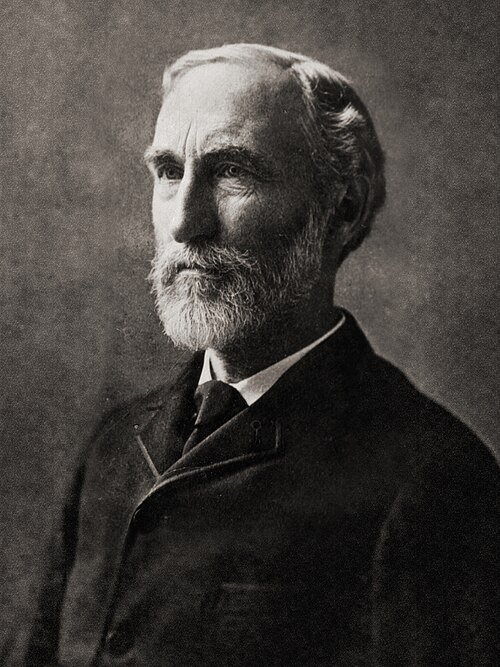
\includegraphics[width=\linewidth]{images/book3/gibbs.jpg}
\end{minipage}\hfill
\begin{minipage}[t]{0.76\linewidth}\vspace{0pt}
Josiah Willard Gibbs (1839--1903), professeur de physique mathématique à
Yale, publia entre 1876 et 1878 \emph{On the Equilibrium of
Heterogeneous Substances}, quelque trois cents pages dans les comptes rendus d'une
petite académie, où apparaissent l'\omterm{def:b2:reaction-free-energy:gibbs-energy}{enthalpie libre}, le potentiel chimique et la
règle des phases des chapitres suivants. Peu de chimistes le lurent avant sa
traduction dans les années 1890. (Photographie~: domaine public, Wikimedia
Commons.)
\end{minipage}
\end{history}

\section{Enthalpies libres standard de réaction et température}

\begin{definition}[Approximation d'Ellingham]\label{def:b2:reaction-free-energy:ellingham-approximation}
L'\emph{approximation d'Ellingham}\index{approximation d'Ellingham} consiste à considérer
$\Delta_r H^\circ$ et $\Delta_r S^\circ$ comme indépendantes de la température
sur un intervalle qui ne contient aucun changement d'état. Alors $\Delta_r G^\circ(T)
= \Delta_r H^\circ - T\Delta_r S^\circ$ est une droite en $T$, de pente
$-\Delta_r S^\circ$.
\end{definition}

\begin{proposition}[Dérivées par rapport à la température]\label{prop:b2:reaction-free-energy:gibbs-helmholtz}
\[
  \frac{\dd\Delta_r G^\circ}{\dd T} = -\Delta_r S^\circ, \qquad
  \frac{\dd}{\dd T}\!\left(\frac{\Delta_r G^\circ}{T}\right) =
  -\frac{\Delta_r H^\circ}{T^2}\ \ \text{(Gibbs--Helmholtz)}, \qquad
  \frac{\dd\Delta_r S^\circ}{\dd T} = \frac{\Delta_r C^\circ_p}{T}.
\]
En particulier, l'\omterm{def:b2:reaction-free-energy:ellingham-approximation}{approximation d'Ellingham} est valable lorsque $\Delta_r C^\circ_p$
est petite.
\end{proposition}

\begin{proof}
Toutes les espèces étant dans leur état standard, $G^\circ(T, \xi)$ vérifie $(\partial
G^\circ/\partial T)_\xi = -S^\circ$ (\cref{prop:b2:reaction-free-energy:dG}).
D'après le théorème de Schwarz,
\[
  \frac{\dd\Delta_r G^\circ}{\dd T} = \partial_\xi\partial_T G^\circ =
  -\partial_\xi S^\circ = -\Delta_r S^\circ .
\] On a alors $\frac{\dd}{\dd
T}(\Delta_r G^\circ/T) = \frac{-T\Delta_r S^\circ - \Delta_r G^\circ}{T^2} =
-\frac{\Delta_r H^\circ}{T^2}$. Enfin, $\dd S^\circ_m = C^\circ_{p,m}\,\dd
T/T$ pour chaque espèce (\cref{prop:b2:reaction-free-energy:absolute-entropy}),
et la même combinaison donne la dernière relation. Si $\Delta_r C^\circ_p$ est
petite, $\Delta_r H^\circ$ (\omterm{thm:b2:reaction-enthalpy:kirchhoff}{loi de Kirchhoff}) et $\Delta_r S^\circ$ varient à peine.
\end{proof}

\begin{definition}[Température d'inversion]\label{def:b2:reaction-free-energy:inversion-temperature}
Lorsque $\Delta_r H^\circ$ et $\Delta_r S^\circ$ ont le même signe, la
\emph{température d'inversion}\index{temperature d'inversion@température d'inversion} de la réaction est
la température où $\Delta_r G^\circ$ change de signe~; dans l'\omterm{def:b2:reaction-free-energy:ellingham-approximation}{approximation
d'Ellingham}, $T_i = \Delta_r H^\circ/\Delta_r S^\circ$.
\end{definition}

\begin{omfigure}
\begin{tikzpicture}
\begin{axis}[
  width=0.72\linewidth, height=5.6cm, xmin=0, xmax=1600, ymin=0, ymax=260,
  axis x line=bottom, axis y line=left, xlabel={$T$ (K)}, ylabel={\unit{kJ/mol}},
  tick label style={font=\small}, label style={font=\small}, clip=false]
\addplot[omThm, very thick] table[x=T, y=DrH] {figdata/out/bachelor-2-thermo-data-calcite.dat};
\addplot[omDef, very thick] table[x=T, y=TDrS] {figdata/out/bachelor-2-thermo-data-calcite.dat};
\node[omThm, anchor=south west, font=\small] at (axis cs:60,180) {$\Delta_r H^\circ = 178.3$};
\node[omDef, anchor=west, font=\small] at (axis cs:1600,257) {$T\Delta_r S^\circ$};
\draw[dotted] (axis cs:1110,0) -- (axis cs:1110,178.3);
\node[anchor=south west, font=\small] at (axis cs:1120,8) {$T_i = \qty{1110}{K}$};
\node[font=\scriptsize, align=center] at (axis cs:600,140) {$\Delta_r G^\circ > 0$~:\\ calcite stable};
\node[font=\scriptsize, align=center] at (axis cs:1470,206) {$\Delta_r G^\circ < 0$};
\end{axis}
\end{tikzpicture}

{\small Terme enthalpique et terme entropique de \ce{CaCO3(s) -> CaO(s) + CO2(g)}
dans l'\omterm{def:b2:reaction-free-energy:ellingham-approximation}{approximation d'Ellingham}. Au-dessous de la \omterm{def:b2:reaction-free-energy:inversion-temperature}{température d'inversion}, le
coût enthalpique l'emporte et le calcaire est stable sous \qty{1}{bar} de dioxyde
de carbone~; au-dessus, le terme entropique l'emporte et le calcaire se décompose.}
% ledger: dfh:CaCO3_cr, dfh:CaO_cr, dfh:CO2, s0:CaCO3_cr, s0:CaO_cr, s0:CO2_g (computed in figdata/bachelor-2/thermo-data.py)
\end{omfigure}

\begin{omfigure}
\begin{tikzpicture}[font=\small]
  \draw[thick] (0,0) rectangle (8,4);
  \draw[thick] (4,0) -- (4,4) (0,2) -- (8,2);
  \node[above] at (2,4) {$\Delta_r H^\circ < 0$};
  \node[above] at (6,4) {$\Delta_r H^\circ > 0$};
  \node[left] at (0,3) {$\Delta_r S^\circ > 0$};
  \node[left] at (0,1) {$\Delta_r S^\circ < 0$};
  \node[align=center, omDef] at (2,3) {exergonique\\ à toute $T$};
  \node[align=center, omProp] at (6,3) {exergonique\\ au-dessus de $T_i$};
  \node[align=center, omProp] at (2,1) {exergonique\\ au-dessous de $T_i$};
  \node[align=center, omThm] at (6,1) {endergonique\\ à toute $T$};
\end{tikzpicture}

{\small Les quatre cas de $\Delta_r G^\circ = \Delta_r H^\circ - T\Delta_r
S^\circ$ (\omterm{def:b2:reaction-free-energy:ellingham-approximation}{approximation d'Ellingham}). Les combustions se trouvent dans la case en haut à gauche~;
la décomposition du calcaire et la poche de froid en haut à droite~; la
synthèse de l'ammoniac en bas à gauche.}
\end{omfigure}

\begin{method}[Une enthalpie libre standard de réaction à la température $T$]\label{met:b2:reaction-free-energy:delta-g-standard}
\begin{enumerate}
  \item À partir des tables à \qty{298.15}{K}, calculer $\Delta_r H^\circ$ et
        $\Delta_r S^\circ$.
  \item Vérifier qu'aucune espèce ne change d'état entre \qty{298}{K} et $T$~;
        sinon, ajouter le changement d'état (enthalpie et entropie) ou partir
        du nouvel état.
  \item Dans l'\omterm{def:b2:reaction-free-energy:ellingham-approximation}{approximation d'Ellingham}, $\Delta_r G^\circ(T) = \Delta_r H^\circ
        - T\Delta_r S^\circ$.
  \item Lorsque $\Delta_r C^\circ_p$ n'est pas petite ou que l'intervalle est long,
        utiliser directement les $\Delta_f G^\circ(T)$ tabulées.
\end{enumerate}
\end{method}

\begin{example}[Deux tests de l'approximation]\label{ex:b2:reaction-free-energy:tests}
Pour le calcaire, $\Delta_r C^\circ_p = 42.80 + 37.13 - 81.88 =
\qty{-2.0}{J/(K.mol)}$~: l'approximation est excellente, et $\Delta_r
G^\circ = 178.3 - T \times 0.1606$ donne $T_i = \qty{1110}{K}$. Pour l'ammoniac,
$\Delta_r G^\circ(700) \approx -91.9 + 700 \times 0.1981 =
\qty{+46.8}{kJ/mol}$, alors que les tables donnent $2\Delta_f G^\circ(\ce{NH3}, 700) =
\qty{+54.4}{kJ/mol}$~: ici $\Delta_r C^\circ_p = \qty{-44}{J/(K.mol)}$, et
l'erreur est de \qty{8}{kJ/mol}, soit un facteur 4 sur la constante d'équilibre à
cette température.
% ledger: cp:CaO_cr.298, cp:CO2_g.298, cp:CaCO3_cr.298, janafG:NH3.700 (computed in figdata/bachelor-2/thermo-data.py)
\end{example}

\section{Exercices}

\begin{exercise}[$\star$]\label{exo:b2:reaction-free-energy:1}
Prévoir le signe de $\Delta_r S^\circ$ pour~: (a) \ce{2H2(g) + O2(g) -> 2H2O(l)}~;
(b) \ce{CaCO3(s) -> CaO(s) + CO2(g)}~; (c) \ce{N2O4(g) -> 2NO2(g)}~;
(d) \ce{Ag+(aq) + Cl-(aq) -> AgCl(s)}~; (e) \ce{H2O(s) -> H2O(l)}~;
(f) \ce{H2(g) + Cl2(g) -> 2HCl(g)}.
\end{exercise}

\begin{exercise}[$\star$]\label{exo:b2:reaction-free-energy:2}
Calculer $\Delta_r S^\circ$ et $\Delta_r G^\circ$ à \qty{298.15}{K} pour la
synthèse de l'ammoniac, \ce{N2(g) + 3H2(g) -> 2NH3(g)}, avec $\Delta_r
H^\circ = \qty{-91.9}{kJ/mol}$ et les entropies du chapitre. Est-elle
\omterm{def:b2:reaction-free-energy:exergonic}{exergonique}~?
\end{exercise}

\begin{exercise}[$\star$]\label{exo:b2:reaction-free-energy:3}
Calculer $\Delta_r G^\circ(\qty{298.15}{K})$ pour \ce{H2(g) + 1/2O2(g) ->
H2O(l)} à partir de $\Delta_f H^\circ(\ce{H2O}, \text{l}) = \qty{-285.83}{kJ/mol}$
et des entropies standard \ce{H2(g)} 130.68, \ce{O2(g)} 205.15,
\ce{H2O(l)} \qty{69.95}{J/(K.mol)}. Pourquoi cette valeur est-elle l'\omterm{def:b2:reaction-free-energy:gibbs-energy}{enthalpie libre}
standard de formation de l'eau liquide~?
% ledger: dfh:H2O-l, s0:H2_g, s0:O2_g, s0:H2O_l
\end{exercise}

\begin{exercise}[$\star$]\label{exo:b2:reaction-free-energy:4}
À l'aide de la figure de l'entropie du zinc, lire son \omterm{def:b2:reaction-free-energy:standard-entropy}{entropie molaire standard} à
\qty{298}{K} et à \qty{1000}{K}, ainsi que ses sauts aux points de fusion et
d'ébullition. En déduire ses enthalpies de fusion et de vaporisation.
\end{exercise}

\begin{exercise}[$\star\star$]\label{exo:b2:reaction-free-energy:5}
Pour \ce{H2O(l) -> H2O(g)} à \qty{298.15}{K}, calculer $\Delta_r H^\circ$,
$\Delta_r S^\circ$ et $\Delta_r G^\circ$ à partir des tables du chapitre.
Expliquer pourquoi $\Delta_r S^\circ \neq \Delta_r H^\circ/T$ à \qty{298}{K} et ce que
signifie la valeur positive de $\Delta_r G^\circ$, puis estimer dans l'\omterm{def:b2:reaction-free-energy:ellingham-approximation}{approximation
d'Ellingham} la température à laquelle l'eau liquide et sa vapeur sous
\qty{1}{bar} sont en équilibre. Comparer à la température d'ébullition.
\end{exercise}

\begin{exercise}[$\star\star$]\label{exo:b2:reaction-free-energy:6}
Pour \ce{N2O4(g) -> 2NO2(g)}, $\Delta_r H^\circ = \qty{57.1}{kJ/mol}$ et
$\Delta_r S^\circ = \qty{175.7}{J/(K.mol)}$. Calculer la \omterm{def:b2:reaction-free-energy:inversion-temperature}{température
d'inversion}, et expliquer pourquoi un tube scellé du gaz brun \ce{NO2} pâlit
lorsqu'on le refroidit dans la glace.
\end{exercise}

\begin{exercise}[$\star\star$]\label{exo:b2:reaction-free-energy:7}
Une réaction a pour $\Delta_r G^\circ = \qty{-12.0}{kJ/mol}$ à \qty{300}{K}
et $\qty{-4.0}{kJ/mol}$ à \qty{400}{K}. Dans l'\omterm{def:b2:reaction-free-energy:ellingham-approximation}{approximation d'Ellingham},
déterminer $\Delta_r H^\circ$ et $\Delta_r S^\circ$, et vérifier la
relation de Gibbs--Helmholtz.
\end{exercise}

\begin{exercise}[$\star\star$]\label{exo:b2:reaction-free-energy:8}
Calculer $\Delta_r G^\circ$ de la formation du méthane, \ce{C(s) + 2H2(g) ->
CH4(g)}, à \qty{298.15}{K}, à partir de $\Delta_f H^\circ = \qty{-74.87}{kJ/mol}$
et des entropies \ce{C} (graphite) 5.74, \ce{H2} 130.68, \ce{CH4}
\qty{186.25}{J/(K.mol)}. Au-dessus de quelle température le méthane devient-il
instable par rapport à ses éléments sous la pression standard~?
% ledger: dfh:CH4_g, s0:C_gr, s0:H2_g, s0:CH4_g
\end{exercise}

\begin{exercise}[$\star\star$]\label{exo:b2:reaction-free-energy:9}
Un halogénoalcane réagit avec une base par substitution ou par élimination. Écrire
les deux réactions pour le 2-bromopropane et l'ion hydroxyde. Avec $\Delta_r
H^\circ(\text{élimination}) - \Delta_r H^\circ(\text{substitution}) =
\qty{+40}{kJ/mol}$ et $\Delta_r S^\circ(\text{élimination}) - \Delta_r
S^\circ(\text{substitution}) = \qty{+90}{J/(K.mol)}$ (ordres de grandeur),
déterminer au-dessus de quelle température l'élimination devient la plus \omterm{def:b2:reaction-free-energy:exergonic}{exergonique} des
deux, et expliquer le rôle du nombre de molécules.
\end{exercise}

\begin{exercise}[$\star\star\star$]\label{exo:b2:reaction-free-energy:10}
Le monoxyde de carbone cristallisé n'atteint pas une entropie nulle à \qty{0}{K}~: chaque
molécule peut se placer en CO ou en OC presque au hasard, les deux orientations ayant
presque la même énergie. En admettant la formule de Boltzmann $S = k_B\ln W$, où
$W$ est le nombre de configurations (dénombrées dans le volume de troisième année), calculer
l'entropie molaire résiduelle. Pourquoi le troisième principe ne s'applique-t-il pas à ce
cristal~?
\end{exercise}

\begin{exercise}[$\star\star\star$]\label{exo:b2:reaction-free-energy:11}
Montrer que si $\Delta_r C^\circ_p$ est une constante $c$,
$\Delta_r S^\circ(T) = \Delta_r S^\circ(T_0) + c\ln(T/T_0)$ et
$\Delta_r G^\circ(T) = \Delta_r H^\circ(T_0) - T\Delta_r S^\circ(T_0) +
c\,[T - T_0 - T\ln(T/T_0)]$. L'appliquer au calcaire ($c =
\qty{-2.0}{J/(K.mol)}$) à \qty{1100}{K}, et mesurer l'erreur de
l'\omterm{def:b2:reaction-free-energy:ellingham-approximation}{approximation d'Ellingham}.
\end{exercise}

\begin{exercise}[$\star\star\star$]\label{exo:b2:reaction-free-energy:12}
On fabrique le titane à partir de son oxyde, le rutile, en passant par son chlorure. (a) Calculer
$\Delta_r H^\circ$ et $\Delta_r S^\circ$ à \qty{298}{K} pour \ce{TiO2(s) +
2Cl2(g) -> TiCl4(g) + O2(g)}, avec \ce{TiO2} ($-944.0$ \unit{kJ/mol},
\qty{50.62}{J/(K.mol)}) et \ce{TiCl4(g)} ($-763.2$, 353.2), puis son
$\Delta_r G^\circ$ à \qty{1000}{K} dans l'\omterm{def:b2:reaction-free-energy:ellingham-approximation}{approximation d'Ellingham}.
(b) On ajoute du carbone~: \ce{C(s) + O2(g) -> CO2(g)}, $\Delta_r H^\circ =
\qty{-393.5}{kJ/mol}$, $\Delta_r S^\circ = \qty{+2.9}{J/(K.mol)}$. Calculer
le $\Delta_r G^\circ(\qty{1000}{K})$ de la somme des deux réactions et
expliquer comment la seconde entraîne la première.
% ledger: dfh:TiO2_cr, s0:TiO2_cr, dfh:TiCl4_g, s0:TiCl4_g, s0:Cl2_g, s0:O2_g, s0:C_gr, s0:CO2_g
\end{exercise}

\section{Problème~: le four à chaux}

\begin{problem}[{Problème du week-end --- l'entropie et l'enthalpie d'une
décomposition, son enthalpie libre en fonction de la température, le critère
d'évolution dans un four, l'énergie et le dioxyde de carbone d'une tonne de
chaux}]
\label{pb:b2:reaction-free-energy:1}
La chaux vive, \ce{CaO}, s'obtient en chauffant du calcaire, \ce{CaCO3}, dans un four. Données à
\qty{298.15}{K}~: $\Delta_f H^\circ$ (\unit{kJ/mol}) \ce{CaCO3(s)}
$-1206.92$, \ce{CaO(s)} $-635.09$, \ce{CO2(g)} $-393.51$~; $S^\circ_m$
(\unit{J/(K.mol)}) 92.9, 39.75, 213.79~; $C^\circ_{p,m}$ (\unit{J/(K.mol)})
81.88, 42.80, 37.13. Masses molaires~: \ce{CaO} \qty{56.08}{g/mol}, \ce{CO2}
\qty{44.01}{g/mol}, \ce{CH4} \qty{16.04}{g/mol}~; combustion du méthane,
eau à l'état de vapeur, $\Delta_r H^\circ = \qty{-802.3}{kJ/mol}$.
% ledger: dfh:CaCO3_cr, dfh:CaO_cr, dfh:CO2, s0:CaCO3_cr, s0:CaO_cr, s0:CO2_g, cp:CaCO3_cr.298, cp:CaO_cr.298, cp:CO2_g.298

\medskip
\noindent\textbf{Partie I --- À température ambiante.}
\begin{enumerate}
  \item Écrire la décomposition du calcaire.
  \item Calculer $\Delta_r H^\circ(\qty{298}{K})$. La réaction est-elle \omterm{def:b2:reaction-enthalpy:exothermic}{exothermique}~?
  \item Calculer $\Delta_r S^\circ(\qty{298}{K})$ et expliquer son signe.
  \item Calculer $\Delta_r G^\circ(\qty{298}{K})$.
  \item Le calcaire est-il stable à température ambiante sous \qty{1}{bar} de
        dioxyde de carbone~? Pourquoi les falaises calcaires durent-elles~?
  \item Calculer $\Delta_r C^\circ_p$, et dire ce qu'il implique pour la
        dépendance en température de $\Delta_r H^\circ$ et de $\Delta_r S^\circ$.
\end{enumerate}

\medskip
\noindent\textbf{Partie II --- Le chauffage.}
\begin{enumerate}[resume]
  \item Écrire $\Delta_r G^\circ(T)$ dans l'\omterm{def:b2:reaction-free-energy:ellingham-approximation}{approximation d'Ellingham}.
  \item La calculer à \qty{1000}{K} et à \qty{1300}{K}.
  \item Calculer la \omterm{def:b2:reaction-free-energy:inversion-temperature}{température d'inversion} $T_i$.
  \item Vérifier la relation de Gibbs--Helmholtz sur cette expression.
  \item Estimer, à l'aide de la formule de l'\cref{exo:b2:reaction-free-energy:11},
        la variation de $\Delta_r G^\circ$ en $T_i$ due à
        $\Delta_r C^\circ_p$, et le déplacement de $T_i$ qui en résulte.
\end{enumerate}

\medskip
\noindent\textbf{Partie III --- Le four.}
Dans cette partie, le dioxyde de carbone au-dessus des solides est sous \qty{1}{bar}, de sorte
que $\Delta_r G = \Delta_r G^\circ$.
\begin{enumerate}[resume]
  \item Que dit le critère d'évolution à \qty{1000}{K}~? Et à
        \qty{1300}{K}~?
  \item Qu'advient-il d'un mélange de chaux vive et de dioxyde de carbone sous
        \qty{1}{bar} refroidi au-dessous de $T_i$~?
  \item Quelle entropie est créée par mole de calcaire décomposé à
        \qty{1300}{K}~?
  \item Les fours sont balayés par les gaz de combustion, plus pauvres en dioxyde de carbone.
        Deviner, avant le chapitre suivant, si cela favorise la
        décomposition.
\end{enumerate}

\medskip
\noindent\textbf{Partie IV --- Une tonne de chaux.}
\begin{enumerate}[resume]
  \item Calculer la quantité de chaux vive dans une tonne.
  \item Calculer la chaleur absorbée par la réaction par tonne de chaux
        (prendre $\Delta_r H^\circ$ constant).
  \item Calculer la masse de dioxyde de carbone libérée par le calcaire par
        tonne de chaux.
  \item La chaleur provient de la combustion du méthane, avec un rendement utile de
        50\,\%. Calculer la masse de méthane brûlée par tonne de chaux.
  \item Calculer le dioxyde de carbone issu de ce méthane.
  \item Calculer le dioxyde de carbone total par tonne de chaux, et la part
        due au calcaire lui-même.
  \item Pourquoi un combustible plus propre ne peut-il réduire qu'une partie de ces émissions~?
  \item Donner la température au-dessus de laquelle le calcaire se décompose sous
        \qty{1}{bar} de dioxyde de carbone.
\end{enumerate}
\end{problem}
